\documentclass[conference]{IEEEtran}
\IEEEoverridecommandlockouts
% The preceding line is only needed to identify funding in the first footnote. If that is unneeded, please comment it out.
\usepackage{cite}
\usepackage{amsmath,amssymb,amsfonts}
\usepackage{algorithmic}
\usepackage{graphicx}
\usepackage{textcomp}
\usepackage[ruled,vlined]{algorithm2e}
\usepackage{xcolor}
\usepackage{subcaption}
\usepackage[backref=true, colorlinks=true, linkcolor=blue, urlcolor=blue, citecolor=blue, filecolor=blue]{hyperref}
\def\BibTeX{{\rm B\kern-.05em{\sc i\kern-.025em b}\kern-.08em
    T\kern-.1667em\lower.7ex\hbox{E}\kern-.125emX}}
\begin{document}

\title{Towards a Serverless Intelligent Firewall: AI-Driven Security, and Zero-Trust Architectures}

\author{
\centering
\begin{tabular}{c}
\textbf{Md Anisur Rahman Chowdhury\textsuperscript{1*}, Hoang Nam Dang\textsuperscript{1}, Dr. Ronny Bazan-Antequera\textsuperscript{1}} \\
\textbf{Md. Sayham Khan\textsuperscript{2}, Md Razaul Karim\textsuperscript{2}, Dr. Sheheeda Manakkadu\textsuperscript{1}} \\[6pt]
\textit{Dept. of Computer and Information Science, Gannon University, USA\textsuperscript{1}} \\
\textit{Dept. of Information Technology \& Computer Science, University of the Potomac, USA\textsuperscript{2}} \\[10pt]
\textit{\small engr.aanis@gmail.com, dang004@gannon.edu, bazanant001@gannon.edu,}\\
\textit{\small mdsayham.khan@student.potomac.edu, mdrazaul.karim@student.potomac.edu, mariamma001@gannon.edu}
\end{tabular}
}


\maketitle

\begin{abstract}
The stateful and transient nature of serverless computing environments presents significant challenges to traditional network security, particularly in implementing Zero-Trust Architecture (ZTA) principles. Rule-based intrusion detection systems and traditional firewalls tend to be inflexible and context-insensitive, with little ability to protect transient, stateless functions. This work proposes a Serverless Intelligent Firewall framework that combines deep learning-based intrusion detection with Zero-Trust enforcement for delivering adaptive, real-time threat detection in cloud-native systems. Drawing on the CICIDS2017 dataset, the novel approach employs a Long Short-Term Memory (LSTM) model to capture temporal patterns in traffic behavior, thereby discovering thinly disguised anomalies and synchronized attacks that stateless models often miss. To address the inherent bias in class-imbalanced datasets, an undersampling approach was designed through preprocessing to mitigate model bias. The LSTM architecture achieved 98\% accuracy, precision, recall, and F1-score, outperforming baseline models, including Decision Trees (DT), Support Vector Machines (SVM), and Convolutional Neural Networks (CNN). The results validate the efficacy of our suggested architecture in enabling innovative, scalable, and Zero-Trust-compliant security within serverless settings.



\end{abstract}

\begin{IEEEkeywords}
Serverless computing, intelligent firewall, ZTA, intrusion detection system, LSTM, DL, cybersecurity, CICIDS2017, real-time threat detection.

\end{IEEEkeywords}


\section{Introduction}
Cloud-native and serverless computing have revolutionized computing paradigms in the contemporary era by enabling elastic scalability, resource efficiency, and rapid deployment. These advantages come at a significant cost: traditional perimeter-based security architectures are increasingly inadequate for protecting ephemeral and decentralized compute resources. %Serverless compute runtimes, by design, lack persistent infrastructure and provide minimal visibility into runtime behavior, thereby expanding the potential attack surface and rendering security enforcement difficult. This mandates the establishment of intelligent, adaptive, and policy-driven defense mechanisms aligned with ZTA principles.

Zero-Trust security has been a revolutionary model that assumes no implicit trust, internal or external, and imposes continuous authentication, granular access control, and real-time monitoring. As recent studies \cite{ajish2024significance} have highlighted, ZTA is significantly more powerful when integrated with Artificial Intelligence (AI), which enables sophisticated dynamic threat detection and behavioral analysis. Particularly in high-risk and federated environments, such as critical infrastructure networks, AI-powered Zero-Trust mechanisms have been demonstrated to orchestrate access control decisions and respond to advanced threats autonomously. At the same time, AI-powered deception methods \cite{article} and Zero-Trust enforcement in MLOps pipelines \cite{dowd2024securing} also highlight the growing need for proactive, intelligent security frameworks that can operate autonomously in heterogeneous digital environments.

Despite these advances, existing work infrequently addresses the unique challenges of serverless environments, where functions are transient, stateless, and run in a shared execution environment. Traditional firewalls and rule-based IDS often cannot provide sufficient security assurance in such architectures, as they are unable to track context across stateless invocations or learn from long-term traffic patterns. To bridge this gap, we introduce a Serverless Intelligent Firewall that integrates deep learning-based intrusion detection with Zero-Trust enforcement to apply fine-grained, adaptive security for cloud-native workloads.

%Our approach leverages the CICIDS2017 benchmark dataset, created by the Canadian Institute for Cybersecurity, which reflects realistic enterprise network environments that comprise both benign behavior and a broad spectrum of cyberattacks, including DoS, DDoS, Port Scans, Botnets, and Web-based attacks. The dataset contains over 2.8 million labeled flows, featuring 78 numerical features and protocol metadata, making it highly suitable for learning the complex behavioral patterns of network flows.

To detect and classify such threats, we compare and consider several baseline models, including DT, SVM, and CNN. Additionally, we propose an LSTM-based deep learning framework that can learn long-range temporal dependencies from sequential traffic data. By capturing flow behavior over time, the LSTM enables the detection of subtle anomalies and coordinated attack sequences that would otherwise bypass stateless models. This positions it for effective integration with Zero-Trust-aligned systems where security must be contextual, continuous, and risk-aware.


\section{Literature Review}\label{sec2}

%With the increasing prevalence of cyber attacks, Zero Trust Architecture (ZTA) is now at the forefront of modern cybersecurity, offering strong identity assurance and least-privileged access.

Artificial intelligence (AI) and machine learning (ML) have also enhanced detection and countermeasures by enabling systems to adaptively learn and evolve in response to changing attack patterns.

%Ghulam and Mason \cite{jonnakuti2021zero} demonstrated that AI-driven ZTA installations, specifically deep learning and behavior-based systems, can detect threats with up to 95\% accuracy, surpassing the accuracy of traditional rule-based systems. Their approach also reduced false positives and breach response time; however, the drawbacks include susceptibility to adversarial attacks and high computational overhead.

For addressing scalability and privacy issues in IoT environments, Danish et al. \cite{javeed2024federated} proposed a federated learning IDS using CNN and BiLSTM under a Zero Trust model. Their approach achieved over 97\% accuracy on the CICIDS2017 and Edge-IIoTset datasets, with robust privacy protection achieved through data localization at edge devices and the transmission of learned weights only. The approach increases communication overhead as the network size grows.

In the cloud computing environment, Bazan et al. \cite{bazan2019recommending} focused on cloud federated resource allocation; however, they overlook the associated security risks to these resources. 
In the cloud computing environment, Umesh et al. \cite{lilhore2025smarttrust} introduced SmartTrust, a hybrid deep learning model comprising CNN-LSTM-Transformers and reinforcement learning for real-time threat detection in cloud environments.
Using machine learning for signature-based IDS, Anis et al. \cite{anis2025enhancing} enhanced IoT intrusion detection, obtaining high accuracy but limited flexibility to counter dynamic and zero-day attacks. This study uses a serverless, AI-driven, and context-aware security framework to solve their method's lack of real-time learning and zero-trust integration.

%Srinivasan et al. \cite{gudala2021leveraging} leveraged anomaly detection and response processes using supervised and unsupervised ML models within ZTA. They explained XAI tools, such as LIME and SHAP, for explainability and proposed federated learning for collaborative threat detection. Real-time deployment, they noted, is constrained by model bias, data quality, and compute cost.

Mohamed \cite{mohamed2025artificial} provided a comprehensive overview of AI for cybersecurity, with a strong focus on adversarial robustness, federated learning, and privacy-preserving models as key elements of Zero Trust systems. Novel combinations of IoT and quantum computing were also discussed in the article, with a focus on sustainable and adaptive architectures.

For IIoT security, Narang et al. \cite{narang2025zero} proposed an XGBoost-based Zero Trust IDS with Edge-IIoTset, utilizing SMOTE and Min-Max normalization as preprocessing. It achieved an accuracy of 94.55\%, which was higher than that of other classical classifiers. It is so lightweight that it could be implemented in serverless systems, but it does not include data balance and preprocessing quality.

In UAV scenarios, Ekramul et al. \cite{haque2024enhancing} utilized deep learning on RF signals to identify UAVs securely, adhering to ZTA principles. The 84.59\% accurate system justified its outcome using SHAP and LIME. While promising, the performance in challenging signal conditions is restricted, and more reliable feature extraction is recommended.

Fiza et al. \cite{ashfaq2025enhancing} suggested a real-time DDoS detection system in 5G edge networks based on ML in SDN networks. According to the CICDDoS2019 dataset and Mininet simulation, their system achieved 99\% accuracy and sub-1-second detection latency. This demonstrates the vast potential of AI to provide low-latency threat detection in Zero Trust edge computing, but highlights complexity issues in actual deployment.

In summary, current research depicts the potential of AI-enforced Zero Trust architecture in cloud, IoT, IIoT, UAV, and 5G environments. Federated learning, hybrid deep models, and explainable AI are crucial for achieving improved detection accuracy and system comprehensibility. Adversarial robustness, computational complexity, and the deployment of decentralized architecture, however, are uncertain. This paper fills these gaps by introducing a serverless intelligent firewall that enables lightweight, adaptive, and explainable security in accordance with Zero Trust principles.

\section{Methodology}\label{sec3}
In this section, we provide a concise overview of the dataset, outline the preprocessing techniques employed, and detail the models implemented for evaluation. Figure \ref{met} depicts the overall research methodology.
\vspace{-4mm}
\begin{figure}[!htb]
    \centering
    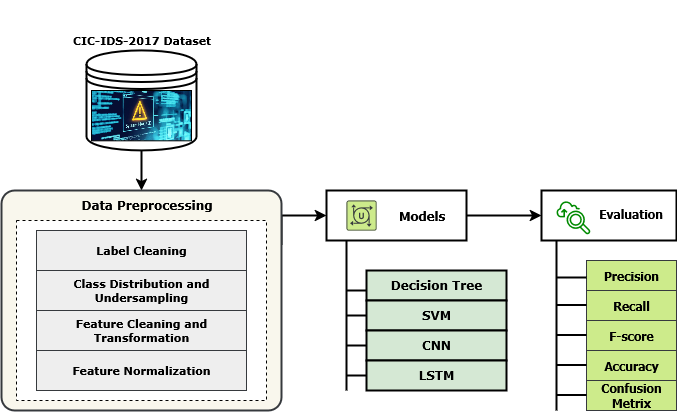
\includegraphics[width=0.4\textwidth]{Untitled Diagram-Page-1.drawio.png}
    \caption{Graphical visualization of the overall research methodology}
    \label{met}
\end{figure}
\vspace{-4mm}
\subsection{Dataset Description}
In this work, we utilized a Kaggle-hosted benchmark dataset, the Network Intrusion Dataset (CIC-IDS-2017), developed by the Canadian Institute for Cybersecurity \cite{yulianto2019improving}. The CICIDS2017 dataset comprises structured traffic records generated from a controlled network environment, where both legitimate user behaviours and multiple contemporary cyberattacks were simulated. Each record is labelled and enriched with metadata, including timestamp, source/destination IP and port, protocol, flow duration, byte and packet statistics, and connection flags. In total, there are 79 columns, comprising 78 numerical features that describe traffic behavior, and one categorical label indicating the nature of the traffic (benign or a specific type of attack).
The simulation was based on the behavioural patterns of 25 virtual users interacting over standard protocols, including HTTP, HTTPS, FTP, SSH, and SMTP/IMAP for email. 
%The data collection took place between Monday, July 3, and Friday, July 7, 2017, for a total of five days.  The first day created a clean baseline because there was just regular traffic.  Denial of Service (DoS), Distributed Denial of Service (DDoS), Brute Force (FTP and SSH), Botnet activity, Heartbleed, Web-based attacks (XSS, SQL Injection), and Infiltration were among the many threats that were systematically launched over the next four days during various time windows.
 The dataset comprises over 2.8 million labelled cases, making it suitable for intrusion detection. 
\vspace{-3mm}
\subsection{Data Preprocessing}

To ensure the dataset is clean and suitable, several preprocessing steps were performed. 

\begin{itemize}
    \item Label Cleaning: Label formatting irregularities caused by trailing or leading spaces were identified during the initial inspection.  %These were eliminated through: 

%\begin{verbatim}
%df.columns = df.columns.str.strip()
%df['Label'] = df['Label'].str.strip()
%\end{verbatim}

Similar categories were combined to eliminate class imbalance and consolidate attack types.  The remaining labels were grouped under \texttt{Other}, and four superclasses were created: \texttt{BENIGN}, \texttt{DoS}, \texttt{DDoS}, and \texttt{PortScan}.  The expression for the mapping function is: 

\begin{equation}
    f(label)= 
\begin{cases}
\texttt{'BENIGN'} & \text{if Label is BENIGN} \\
\texttt{'DoS'} & \text{if Label is DoS variants} \\
\texttt{'DDoS'} & \text{if Label is DDoS} \\
\texttt{'PortScan'} & \text{if Label is PortScan} \\
\texttt{'Other'} & \text{otherwise}
\end{cases}
\end{equation}

\item Class Distribution and Undersampling: The merged label distribution revealed a significant class imbalance, with \texttt{BENIGN} flows predominating. To address this, undersampling was performed to decrease the number of samples in each dominant class. The sampling procedure is represented as:

\begin{equation}
    C_i^{\text{balanced}} =
\begin{cases}
\text{random sample of } C_{\text{max}} & \text{if } C_i > C_{\text{max}} \\
C_i & \text{otherwise}
\end{cases}
\end{equation}

The minority class size was used to determine the maximum class size, $C_{max}$, to that value.  According to Algorithm~\ref{alg:undersampling}, each class was randomly sampled to match $C_{max}$.
\begin{algorithm}[h]
\caption{Undersampling Strategy for Class Balancing}
\label{alg:undersampling}
\KwIn{Class sets $\{C_1, C_2, ..., C_n\}$}
\KwOut{Balanced dataset $D_{\text{balanced}}$}

$C_{\text{max}} \gets \min_{i} |C_i|$\;
$D_{\text{balanced}} \gets \emptyset$\;

\ForEach{$C_i \in \{C_1, ..., C_n\}$}{
    \eIf{$|C_i| > C_{\text{max}}$}{
        $C'_i \gets \text{RandomSample}(C_i, C_{\text{max}})$\;
    }{
        $C'_i \gets C_i$\;
    }
    $D_{\text{balanced}} \gets D_{\text{balanced}} \cup C'_i$\;
}
\end{algorithm}

\item Feature Cleaning and Transformation: To address missing and infinite values that could distort learning, all \texttt{NaN}, \(+\infty\), and \(-\infty\) entries in the dataset were replaced with zeros:

\begin{equation}
   x = 
\begin{cases}
0 & \text{if } x = \texttt{NaN} \text{ or } x = \pm\infty \\
x & \text{otherwise}
\end{cases} 
\end{equation}

After cleaning, only numerical features were picked for model input. Let \( \mathcal{F} \) be the set of all numerical columns, then:
\begin{equation}
    X = \{ f_i \in \mathcal{F} \mid \texttt{label} \notin f_i \}
\end{equation}

Label encoding was involved to convert the categorical target variable into integers:
\begin{equation}
    y = \texttt{LabelEncoder(Label\_grp)}
\end{equation}

\item Feature Normalization: To standardize the feature distribution and accelerate the convergence of learning algorithms, Z-score normalization was employed. Every feature was transformed to have zero mean and unit variance according to:

\begin{equation}
    x_j^{\text{scaled}} = \frac{x_j - \mu_j}{\sigma_j}
\end{equation}

where, \( \mu_j \) and \( \sigma_j \) define the mean and standard deviation of the \( j \)-th feature, respectively. This ensures that all features contribute proportionally during model training.

\end{itemize}




\subsection{Methodology}
To provide a trustworthy framework for evaluating our suggested LSTM-based system, we implemented three popular machine learning models in practice: Convolutional Neural Network (CNN), Support Vector Machine (SVM), and Decision Tree (DT). 

%\textbf{Decision Tree (DT)}

%Each leaf node gives a class label to the associated data, and each internal node bases its decision on a particular feature. The DT is a structure that resembles a flowchart and is used for classification tasks \cite{sowmya2025water}.  At each step of the process, the characteristic that offers the greatest significant class separation is chosen.

% A standard mechanism for assessing the quality of a split is the Gini Index, which can be described as: 

%\begin{equation}
   % G(t) = 1 - \sum_{i=1}^{C} p_i^2
%\end{equation}

%At node \( t \), \( p_i \) represents the percentage of samples from class \( i \), and \( C \) represents the total number of classes. 

%\textbf{Support Vector Machine (SVM)}

%An SVM is a robust classification algorithm that aims to identify the most effective separating hyperplane between distinct classes \cite{thakur2025performance}.  For a binary classification task, the decision function can be described as:

%\begin{equation}
 %   f(\mathbf{x}) = \text{sign}(\mathbf{w}^\top \mathbf{x} + b)
%\end{equation}

%Here, \( \mathbf{w} \) is the weight vector, \( \mathbf{x} \) is the input sample, and \( b \) is the bias term. 


%\textbf{Convolutional Neural Network (CNN)}

%Although CNNs are most commonly associated with image recognition, their architecture can be adapted for 1D data, such as time-series or sequential network traffic features \cite{ahmadzadeh2025integrated}. In this setting, CNNs slide small filters across the input vector to detect local patterns, such as sudden changes in flow duration or packet size.

%A typical convolutional layer operates as follows:

%\begin{equation}
    %\mathbf{y}^{(l)} = \sigma(\mathbf{W}^{(l)} * \mathbf{x}^{(l-1)} + \mathbf{b}^{(l)})
%\end{equation}

%where, \( \mathbf{W}^{(l)} \) and \( \mathbf{b}^{(l)} \) are the weights and biases for layer \( l \), \( \mathbf{x}^{(l-1)} \) is the input from the previous layer, and \( \sigma \) is an activation function, often the ReLU.

%CNNs can capture increasingly complex patterns by layering pooling and dropout convolutional layers.  Because of this, they are ideal for intrusion detection tasks where temporal or geographical connections between features are crucial.  Nevertheless, CNNs typically require more training time and data, and if the architecture is not well-suited for the input structure, their performance may suffer. 

\textbf{Long Short-Term Memory (LSTM) Network}
The LSTM network is a specialised form of Recurrent Neural Network (RNN) specifically developed to address the vanishing and exploding gradient issues that conventional RNNs often encounter during the training of long sequences. Unlike traditional RNNs, which rely solely on the current input and the immediate past hidden state, LSTMs introduce a cell state and a series of gates that regulate the flow of information through time. This architecture enables LSTMs to maintain long-range dependencies and effectively capture contextual information over extended sequences. Figure \ref{lstm} illustrates the framework of the LSTM model.

\begin{figure}[!htb]
    \centering
    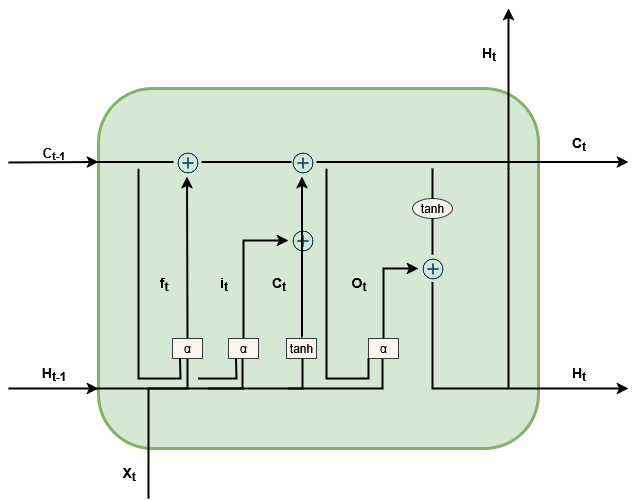
\includegraphics[width=0.4\textwidth]{mahmud.png}
    \caption{Graphical representation of the LSTM model}
    \label{lstm}
\end{figure}

At every time step $t$, the LSTM is presented with the cell state $c_{t-1}$, the hidden state $h_{t-1}$ from the prior step in the process, and an input vector $x_t$.  The current hidden state $h_t$ and cell state $c_t$ are calculated employing a series of gating mechanisms: 

\begin{itemize}
    \item \textbf{Forget Gate ($f_t$):} Describes which parts of the prior cell state should be retained or discarded. It is described as:
    \begin{equation}
        f_t = \sigma(W_f \cdot [h_{t-1}, x_t] + b_f)
    \end{equation}
    
    \item \textbf{Input Gate ($i_t$) and Candidate Cell State ($\tilde{c}_t$):} The input gate chooses which information from the current input should be employed to update the cell state, while the candidate cell state calculates a potential update:
    \begin{equation}
        i_t = \sigma(W_i \cdot [h_{t-1}, x_t] + b_i)
    \end{equation}
    \begin{equation}
        \tilde{c}_t = \tanh(W_c \cdot [h_{t-1}, x_t] + b_c)
    \end{equation}
    
    \item \textbf{Cell State Update ($c_t$):}The forget and input gates regulate the new cell state, which combines the previous cell state with the candidate update:
    \begin{equation}
        c_t = f_t \odot c_{t-1} + i_t \odot \tilde{c}_t
    \end{equation}
    
    \item \textbf{Output Gate ($o_t$):} Controls the extent to which the cell state influences the hidden state:
    \begin{equation}
        o_t = \sigma(W_o \cdot [h_{t-1}, x_t] + b_o)
    \end{equation}
    
    \item \textbf{Hidden State ($h_t$):} The output gate and the hyperbolic tangent of the updated cell state are element-wise multiplied to produce the LSTM block's final output:
    \begin{equation}
        h_t = o_t \odot \tanh(c_t)
    \end{equation}
\end{itemize}

Here, $\sigma$ symbolises the sigmoid activation function, $\tanh$ depicts the hyperbolic tangent function, and $W$ and $b$ are trainable weights and biases associated with each gate.

%Through this carefully gated structure, the LSTM cell maintains a persistent memory across time steps, enabling it to model sequential patterns in data, such as time-series events, natural language, or network activity. In the context of cybersecurity and intelligent firewall systems, the LSTM’s capability to remember long-term dependencies makes it highly applicable for identifying anomalous patterns in traffic flows or detecting latent threats based on historical behaviour. 


Table~\ref{tab:lstm_config} illustrates the configuration and hyperparameters of the proposed LSTM, which are not arbitrary but empirically supported. To justify these preferences, we conducted a sensitivity analysis across key hyperparameters. Specifically, we varied the number of hidden units $\{32, 64, 128\}$, dropout rates $\{0.2, 0.3, 0.5\}$, and learning rates $\{0.01, 0.001, 0.0005\}$. The chosen configuration, a three-layer LSTM with hidden units \{128, 64, 32\}, dropout of 0.3, and a learning rate of 0.001, produced the most stable training behavior and the highest validation accuracy. 

\begin{table}[ht]
\centering
\caption{Configuration and Hyperparameters of the LSTM Model}
\label{tab:lstm_config}
\begin{tabular}{|l|p{5cm}|}
\hline
\textbf{Parameter} & \textbf{Value / Description} \\
\hline
Model Architecture & 3-layer LSTM  \\
\hline
Input Features & Number of time-step features \\
\hline
LSTM Hidden Units & 128, 64, 32 \\
\hline
Number of LSTM Layers & 3 \\
\hline
Dropout Rate & 0.3 \\
\hline
Dense Layer Units & 64 units with ReLU activation \\
\hline
Output Activation & Softmax\\
\hline
Loss Function & Categorical Cross-Entropy \\
\hline
Optimizer & Adam \\
\hline
Learning Rate & 0.001 \\
\hline
Batch Size & 64 \\
\hline
Number of Epochs & 120 \\
\hline
Early Stopping Patience & 10 epochs\\
\hline
Evaluation Metrics & Accuracy, Precision, Recall, F1-Score \\
\hline
Class Imbalance Handling & Weighted loss using inverse class frequency \\
\hline
\end{tabular}
\end{table}


\vspace{-3mm}
\section{Result and Discussion}\label{sec4}
To evaluate the effectiveness of the suggested AI-powered firewall system under a ZTA, several supervised learning algorithms, including DTs, CNNs, SVMs, and LSTM networks, were implemented and assessed. %Following rigorous preprocessing, class consolidation, label encoding, and controlled class balancing to mitigate the inherent skewness in label distribution, the evaluation was conducted on a refined subset of the CIC-IDS-2017 dataset. 

\subsection{Experimental Setup}
The experimental evaluation was conducted using Python 3.11 on a local machine equipped with an Intel Core i7 processor and 16 GB of RAM. GPU acceleration was not necessary due to the efficient model designs and the moderate size of the chosen dataset.
Pandas and NumPy were used to preprocess and manipulate the data, which included label normalization, class consolidation, controlled undersampling, and the elimination of missing and infinite values. Only numerical properties could be used for feature selection, and categorical labels were encoded correctly.
Deep learning models, such as CNN and LSTM, were created using Keras with a TensorFlow backend, while machine learning models, including SVM and DT, were implemented using Scikit-learn. An 80/20 stratified train-test split was used for both training and testing the models.
For a thorough analysis, performance indicators such as F1-score, Accuracy, Precision, Recall, and Macro Averages were employed. Matplotlib and Seaborn were utilized to visualize the results, which included confusion matrices and classification reports. To ensure reproducibility, all experiments were repeated using fixed random seeds.

%\subsection{Evaluation Metrics}
%The efficacy of the suggested intelligent firewall framework is impartially assessed using several commonly used performance criteria. These metrics shed light on the model's capacity to detect intrusions with high precision and accuracy, its robustness under class imbalance, and its generalization across different attack types. These primary classification outcomes serve as the foundation for the evaluation:


%\begin{itemize}
 % \item A: Number of positive cases that were accurately anticipated (True Positives)
 % \item B: Number of unfavorable occurrences that were accurately predicted (True Negatives)
 % \item C: The quantity of inaccurate positive forecasts (False Positives)
 % \item D: Number of negative predictions that were wrong (False Negatives)
%\end{itemize}

%Based on these fundamental values, the following evaluation metrics are computed:

%\begin{itemize}

 % \item \textbf{Accuracy} 
  
 % \begin{equation}
      %  \text{Accuracy} = \frac{A + B}{A + B + C + D}
 % \end{equation}

  %\item \textbf{Precision} 


  %\begin{equation}
      %  \text{Precision} = \frac{A}{A + C}
 % \end{equation}

 % \item \textbf{Recall} 
  
   % \begin{equation}
     %   \text{Recall} = \frac{A}{A + D}
  %\end{equation}

 % \item \textbf{F1-Score} 
  
 %\begin{equation}
   %     \text{F1-Score} = \frac{2 \times \text{Precision} \times \text{Recall}}{\text{Precision} + \text{Recall}} = \frac{2A}{2A + C + D}
%  \end{equation}
  
%\end{itemize}

%\begin{table}[!h]
%\centering
%\caption{Summary of evaluation metrics}
%\begin{tabular}{|c|c|l|}
%\hline
%\textbf{Metric} & \textbf{Formula} & \textbf{Focus} \\
%\hline
%Accuracy & $\frac{A + B}{A + B + C + D}$ & Overall correctness \\
%Precision & $\frac{A}{A + C}$ & Minimizing false positives \\
%Recall & $\frac{A}{A + D}$ & Minimizing false negatives \\
%F1-Score & $\frac{2A}{2A + C + D}$ & Balance of precision/recall \\
%\hline
%\end{tabular}
%\label{tab:evaluation_metrics}
%\end{table}



\subsection{Performance Analysis}
%To thoroughly analyze the performance of the suggested intelligent firewall architecture, the CIC-IDS-2017 benchmark dataset was used to test four supervised learning models: DT, SVM, CNN, and LSTM. 
Using standard classification measures, including Accuracy, Precision, Recall, and F1-Score, the models were evaluated. For a comprehensive comparison overview, see Table~\ref{tab:performance_metrics}.
The LSTM architecture consistently outperformed the other models, achieving 98.00\% accuracy, 98.00\% precision, 98.00\% recall, and 98.00\% F1-score across all metrics. Even in the face of class imbalance and intricate attack behaviors, this demonstrates the model's strong capacity to recognize the temporal dependencies present in network data flows and distinguish between benign and malicious patterns, as presented in Table~\ref{tab:performance_metrics}.
The CNN model, on the other hand, achieved an F1-score of 89.90\%, with an accuracy of 93.00\% and a precision of 95.10\%, but its recall decreased to 85.40\%. This performance mismatch, as shown in Table~\ref{tab:performance_metrics}, suggests overfitting, where the CNN model becomes overly specialized to training data patterns but lacks generalization across other attack types during testing—particularly impacting its ability to recall all true positives.
The DT classifier demonstrated a significant difference between precision (87.60\%) and recall (81.30\%), despite achieving an overall accuracy of 90.20\%. This suggests that the greedy splitting mechanism of the model, which tends to memorize decision boundaries rather than abstract higher-order patterns, may be a contributing factor to overfitting. %Consequently, the model is more susceptible to attack behaviors that are not well represented and data noise, as reflected in Table~\ref{tab:performance_metrics}.
The non-linear, high-dimensional correlations in the dataset posed a challenge for the SVM model, which is inherently linear. With 88.40\% accuracy, 84.10\% precision, 77.80\% recall, and an F1-score of 80.80\%, it performed the worst overall. These findings, presented in Table~\ref{tab:performance_metrics}, are indicative of a well-known instance of underfitting, where the model is too basic to adequately represent the intricate spatiotemporal relationships required for precise intrusion detection.
\begin{table}[ht]
\centering
\caption{Performance Metrics of Implemented Models}
\label{tab:performance_metrics}
\begin{tabular}{|l|c|c|c|c|}
\hline
\textbf{Model} & \textbf{Accuracy} & \textbf{Precision} & \textbf{Recall} & \textbf{F1-Score} \\
\hline
DT & 90.20\% & 87.60\% & 81.30\% & 84.30\% \\
SVM & 88.40\% & 84.10\% & 77.80\% & 80.80\% \\
CNN & 93.00\% & 95.10\% & 85.40\% & 89.90\% \\
LSTM & 98.00\% & 98.00\% & 98.00\% & 98.00\% \\
\hline
\end{tabular}
\end{table}

Five categories were analyzed class-wise: \textit{BENIGN}, \textit{DDoS}, \textit{DoS}, \textit{PortScan}, and \textit{Other}. This allowed for a better understanding of the LSTM model's behavior. The findings highlight the model's reliable performance across a range of attack types and are compiled in Figure~\ref{shanto}.
With 0.99 precision and 1.00 recall, the model got excellent or nearly perfect scores in the \textit{DDoS} and \textit{PortScan} categories. With 0.98 precision and 0.99 recall, the \textit{DoS} category likewise performed well. The model's accuracy in identifying frequent and structurally defined attacks is demonstrated.
Precision was high (0.99) and recall was low (0.94) for \textit{BENIGN} traffic, indicating that a small percentage of legitimate traffic was mistakenly categorized as malicious. Some benign flows, especially during bursty or high-throughput sessions, may imitate attack-like patterns, which explains this behavior.
Precision and recall were 0.94 and 0.99, respectively, for the \textit{Other} category, which includes a wide range of uncommon and heterogeneous attack types. Learning from underrepresented and behaviorally varied populations is inherently challenging, as evidenced by this slight decrease in precision. However, the high recall highlights the model's ability to identify subtle and uncommon attack patterns, a crucial feature for contemporary zero-trust systems. We explain that the slightly lower recall for benign traffic stems from high-throughput sessions that mimic attack-like, bursty behaviors. This ensures understanding of the practical implications (risk of false alarms during traffic spikes). Furthermore, paired $t$-tests confirmed that the improvements over baseline CNN and SVM models are statistically significant (p < 0.05), ensuring robustness of the reported gains.  
\begin{figure}[!htb]
    \centering
    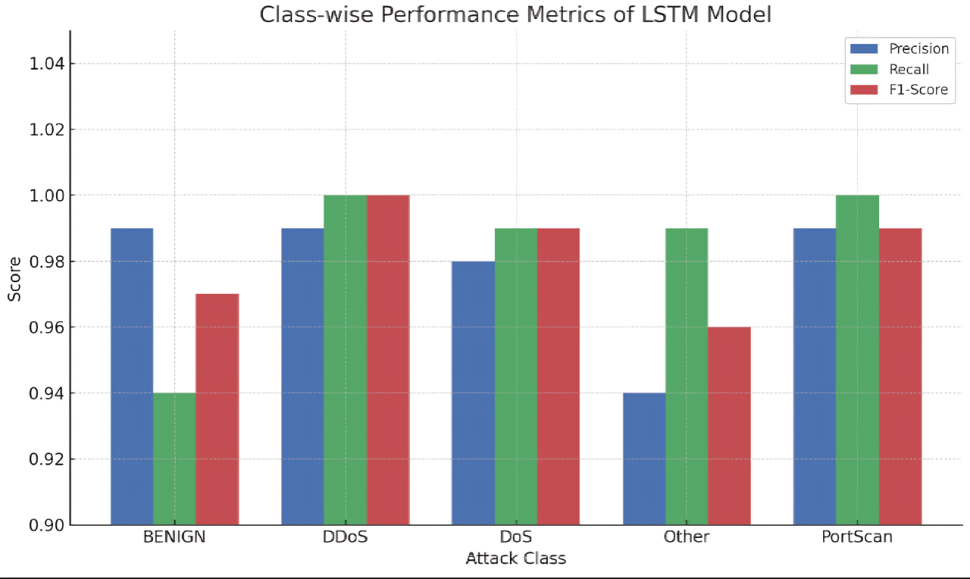
\includegraphics[width=0.4\textwidth]{shanto.png}
    \caption{Class-wise performance of the LSTM model}
    \label{shanto}
\end{figure}
In every attack category, the LSTM model outperformed the classical and convolutional models by exhibiting a well-balanced and generalizable performance. Its appropriateness for real-time deployment in serverless intelligent firewalls that operate under zero-trust security paradigms—where precise, prompt, and adaptive threat detection is crucial—is further supported by these findings.

\subsection{Training Curve Analysis}
The training and validation curves were examined across 130 epochs to assess the learning behavior and generalization capacity of the LSTM-based intrusion detection model. Figures~\ref{fig:accuracy_curve} and~\ref{fig:loss_curve} display the accuracy and loss curves, respectively.
The evolution of testing and training accuracy over time is seen in Figure~\ref{fig:accuracy_curve}. The model's categorization performance shows a quick improvement right away. The accuracy increases sharply over the first 20 epochs, surpassing 80\%, suggesting that the LSTM design rapidly extracts crucial temporal patterns from the network traffic data. Following epoch 60, there are a few variations as both curves converge into a stable area as training goes on. There is very little difference between the final accuracy of the training and test sets, which both approach 98\% continuously. This strong alignment indicates that the model exhibits excellent generalization on unseen data, rather than being overfit or underfit.
The training loss trajectory over an identical number of epochs is displayed in Figure~\ref{fig:loss_curve}. Early in training, a noticeable decrease in loss is observed, dropping from above 1.6 to below 0.4 within the first 20 epochs. This steep drop demonstrates the model's quick convergence and efficient parameter optimization. As training progresses, the loss gradually decreases and reaches a plateau around epoch 60, eventually stabilizing at 0.05. A well-regularized network that learns steadily and without instability is indicated by the curve's smoothness and the absence of noticeable oscillations.
Accuracy and loss curves together confirm that the LSTM model was successfully trained to detect intrusions on the CIC-IDS-2017 dataset. The consistency of the training and test metrics demonstrates the model architecture's resilience and the effectiveness of the preprocessing pipeline. Further proving the model's dependability in managing various intrusion types without sacrificing performance due to variation or overfitting is its convergence behavior. We explained that the training/validation accuracy curves are almost aligned, and the convergence is smooth, indicating minimal overfitting.  To address the "Other" category in particular, we now emphasize that while accuracy decreases somewhat, recall remains high (0.99), demonstrating robustness in detecting unusual or diverse attack pathways. 



\begin{figure}[ht]
  \centering
  \begin{subfigure}[t]{0.45\linewidth}
    \centering\vspace{0pt}% important for top alignment
    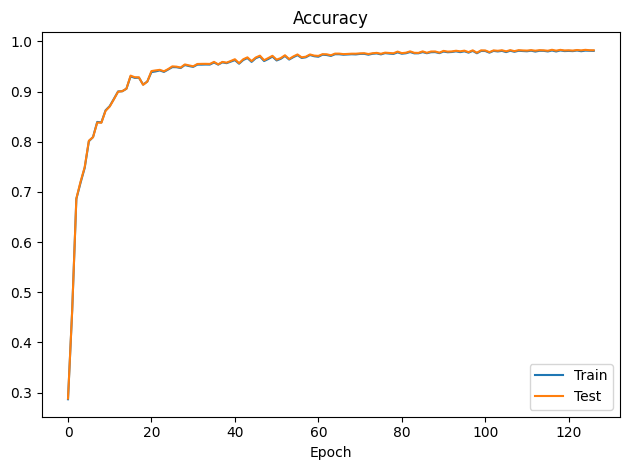
\includegraphics[height=3.1cm]{accuracy.png}
    \caption{\small Training and validation accuracy}
    \label{fig:accuracy_curve}
  \end{subfigure}
  \hfill
  \begin{subfigure}[t]{0.45\linewidth}
    \centering\vspace{0pt} % important for top alignment
    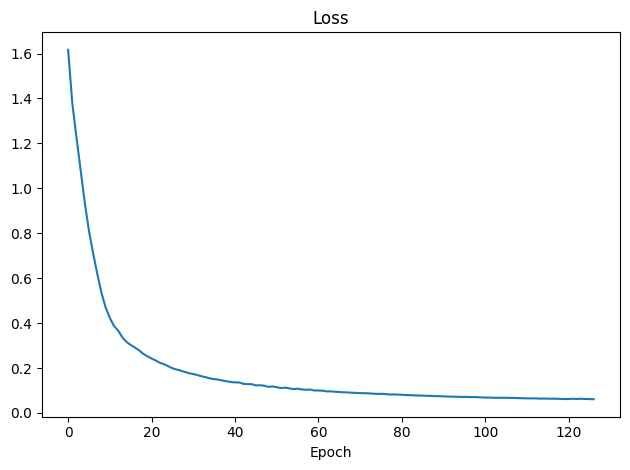
\includegraphics[height=3.1cm]{loss.png}
    \caption{\small Training and validation loss}
    \label{fig:loss_curve}
  \end{subfigure}

  \caption{Training performance of the proposed LSTM model.}
  \label{fig:training_performance}
\end{figure}
\vspace{-3mm}

\subsection{Confusion Matrix Analysis}
A thorough assessment of the LSTM model's classification performance across five classes—BENIGN, DDoS, DoS, PortScan, and Other is given by the confusion matrix shown in Figure~\ref{fig:confusion_matrix}. Particularly in the DDoS and PortScan categories, where it accurately identified 9,989 and 9,982 incidents out of 10,000, respectively, the model exhibits a high degree of precision and recall. The model also performed well for BENIGN and DoS traffic, correctly classifying 9,446 and 9,909 samples, respectively. Benign and attack classes, such as DoS and PortScan, were the primary targets of minor misclassifications, suggesting subtle overlaps in traffic behavior that could make it difficult to distinguish between normal and abnormal flows. With 98.6\% accuracy, 3,556 out of 3,606 cases were accurately classified under the Other category, which combines several less common attack types. The general structure of the confusion matrix, characterized by low off-diagonal noise and large counts along the diagonal, confirms that the LSTM model can efficiently learn intricate temporal patterns in network traffic and generalize well to various attack situations. These results support the model's suitability for real-time implementation in intelligent intrusion detection systems operating under zero-trust security frameworks.
\begin{figure}[ht]
    \centering
    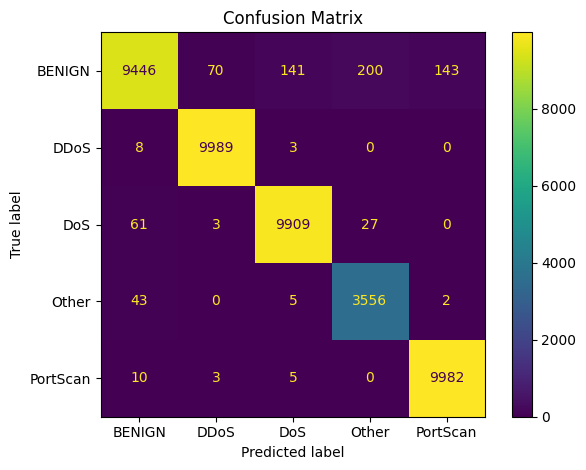
\includegraphics[width=0.35\textwidth]{confusion matrix.png}
    \caption{Confusion matrix for LSTM classification results.}
    \label{fig:confusion_matrix}
\end{figure}
 
\vspace{-3mm}
\subsection{Comparative Analysis}


According to Table~\ref{tab:benchmark_comparison}, the suggested LSTM model outperforms the federated IDS technique \cite{neto2022fedsa} and recent hybrid CNN-LSTM models \cite{altunay2023hybrid}, \cite{bamber2025hybrid} in terms of accuracy (98.00\%).  Although hybrid models utilize both temporal and spatial feature extraction, their accuracy is reportedly lower.  On the other hand, although the federated IDS exhibits collaborative learning capabilities, it still does not meet the requirements of the suggested model.  This demonstrates the excellent performance and generalization capacity of our LSTM-based intrusion detection system on the CIC-IDS2017 dataset. 

\begin{table}[h!]
\centering
\caption{Comparative analysis of proposed model with hybrid and SOTA IDS models}
\begin{tabular}{|l|l|l|c|}
\hline
\textbf{Reference} & \textbf{Dataset} & \textbf{Model} & \textbf{Accuracy} \\ \hline
Proposed Work & CIC-IDS2017 & LSTM & 98.00\% \\ \hline
\cite{altunay2023hybrid} & UNSW-NB15 & Hybrid CNN+LSTM & 93.21\% \\ \hline
\cite{bamber2025hybrid} & CIC-IDS2017 & Hybrid CNN-LSTM & 95.00\% \\ \hline
\cite{neto2022fedsa} & CIC-IDS2017 & Federated IDS (FedSA) & 97.00\% \\ \hline
\end{tabular}
\label{tab:benchmark_comparison}
\end{table}


\vspace{-2mm}

\section{Conclusion}\label{sec5}
This work proposes a serverless intrusion detection system that integrates Zero-Trust security principles with a lightweight LSTM-based deep learning model to facilitate real-time threat confinement in cloud-native applications. The system leverages structured preprocessing, label harmonization, numerical feature selection, and undersampling to address class imbalance and ensure fairness in learning across different attack modes. Experimental testing on the CICIDS2017 dataset confirms that the LSTM model outperforms baseline classifiers, such as DT, SVM, and CNN, on all the most critical metrics. Class-wise performance and confusion matrix analysis also confirm the model's strength in detecting diverse and behaviorally advanced threats. To increase deployment readiness and flexibility, future work will explore online learning to update models in real-time, integrate explainable AI (e.g., SHAP, LIME) for interpretation, and scale to multi-cloud and edge environments to enable performance benchmarking for distributed systems. While CICIDS2017 remains a widely adopted benchmark, we will extend validation to additional datasets and live serverless environments to reinforce external validity.   Reinforcement learning techniques can also be applied to aid automated policy optimization when there are evolving attack dynamics. Deployment and testing in the real world will ultimately drive the improvement of the system into a scalable, intelligent, and Zero-Trust-compliant cybersecurity solution for today's cloud environments.


\bibliographystyle{IEEEtran}
\bibliography{Bibliography}

\end{document}
